\chapter{The Compact Muon Solenoid}
\label{chap:detector}

\section{Introduction}

The Large Hadron Collider (LHC) at CERN is a 27\,km hadron accelerator and collider with a design centre-of-mass energy of 14\,TeV~\cite{LHC}.
Its purpose is to provide collisions sufficient in energy and number to precisely probe physics at the electroweak scale.
Four detectors, one of which is the Compact Muon Solenoid (CMS), are situated around the LHC ring.
CMS is a general-purpose detector designed to precisely measure a wide range of physics objects.
Together, the LHC and CMS facilitate a wide-ranging program of physics studies, from SM precision measurements to dark matter searches, 
and including exploration of electroweak symmetry breaking via production of the Higgs boson.
This chapter will describe the design and operation of both the LHC and the CMS detector.

\section{The Large Hadron Collider}

The LHC is situated in the tunnel that previously housed the Large Electron Positron collider (LEP), 
around 100\,m below ground across the French-Swiss border near CERN.
It is the final machine in a series of accelerators which form the CERN accelerator complex; 
these  act as the injection system for the LHC.
The two counter-circulating beams cross at four interaction points, at each of which a detector is situated.
Directly opposite CMS is a second general purpose detector, ATLAS~\cite{ATLAS}, 
whose physics objectives are identical to those of CMS but with different design decisions.
The other two detectors, LHCb~\cite{LHCb} and ALICE~\cite{ALICE}, focus on flavour and heavy-ion physics respectively.
Whilst the LHC is capable of producing heavy ion collisions in addition to proton-proton collisions, 
the remainder of this section will be dedicated to its proton-proton operations.
A schematic of the full CERN accelerator complex and the LHC experiments is shown in Figure~\ref{fig:detector_CERNschematic}.
The operation of the LHC and the data it has accumulated so far is described in detail below.

\begin{figure}[h!]
  \centering
  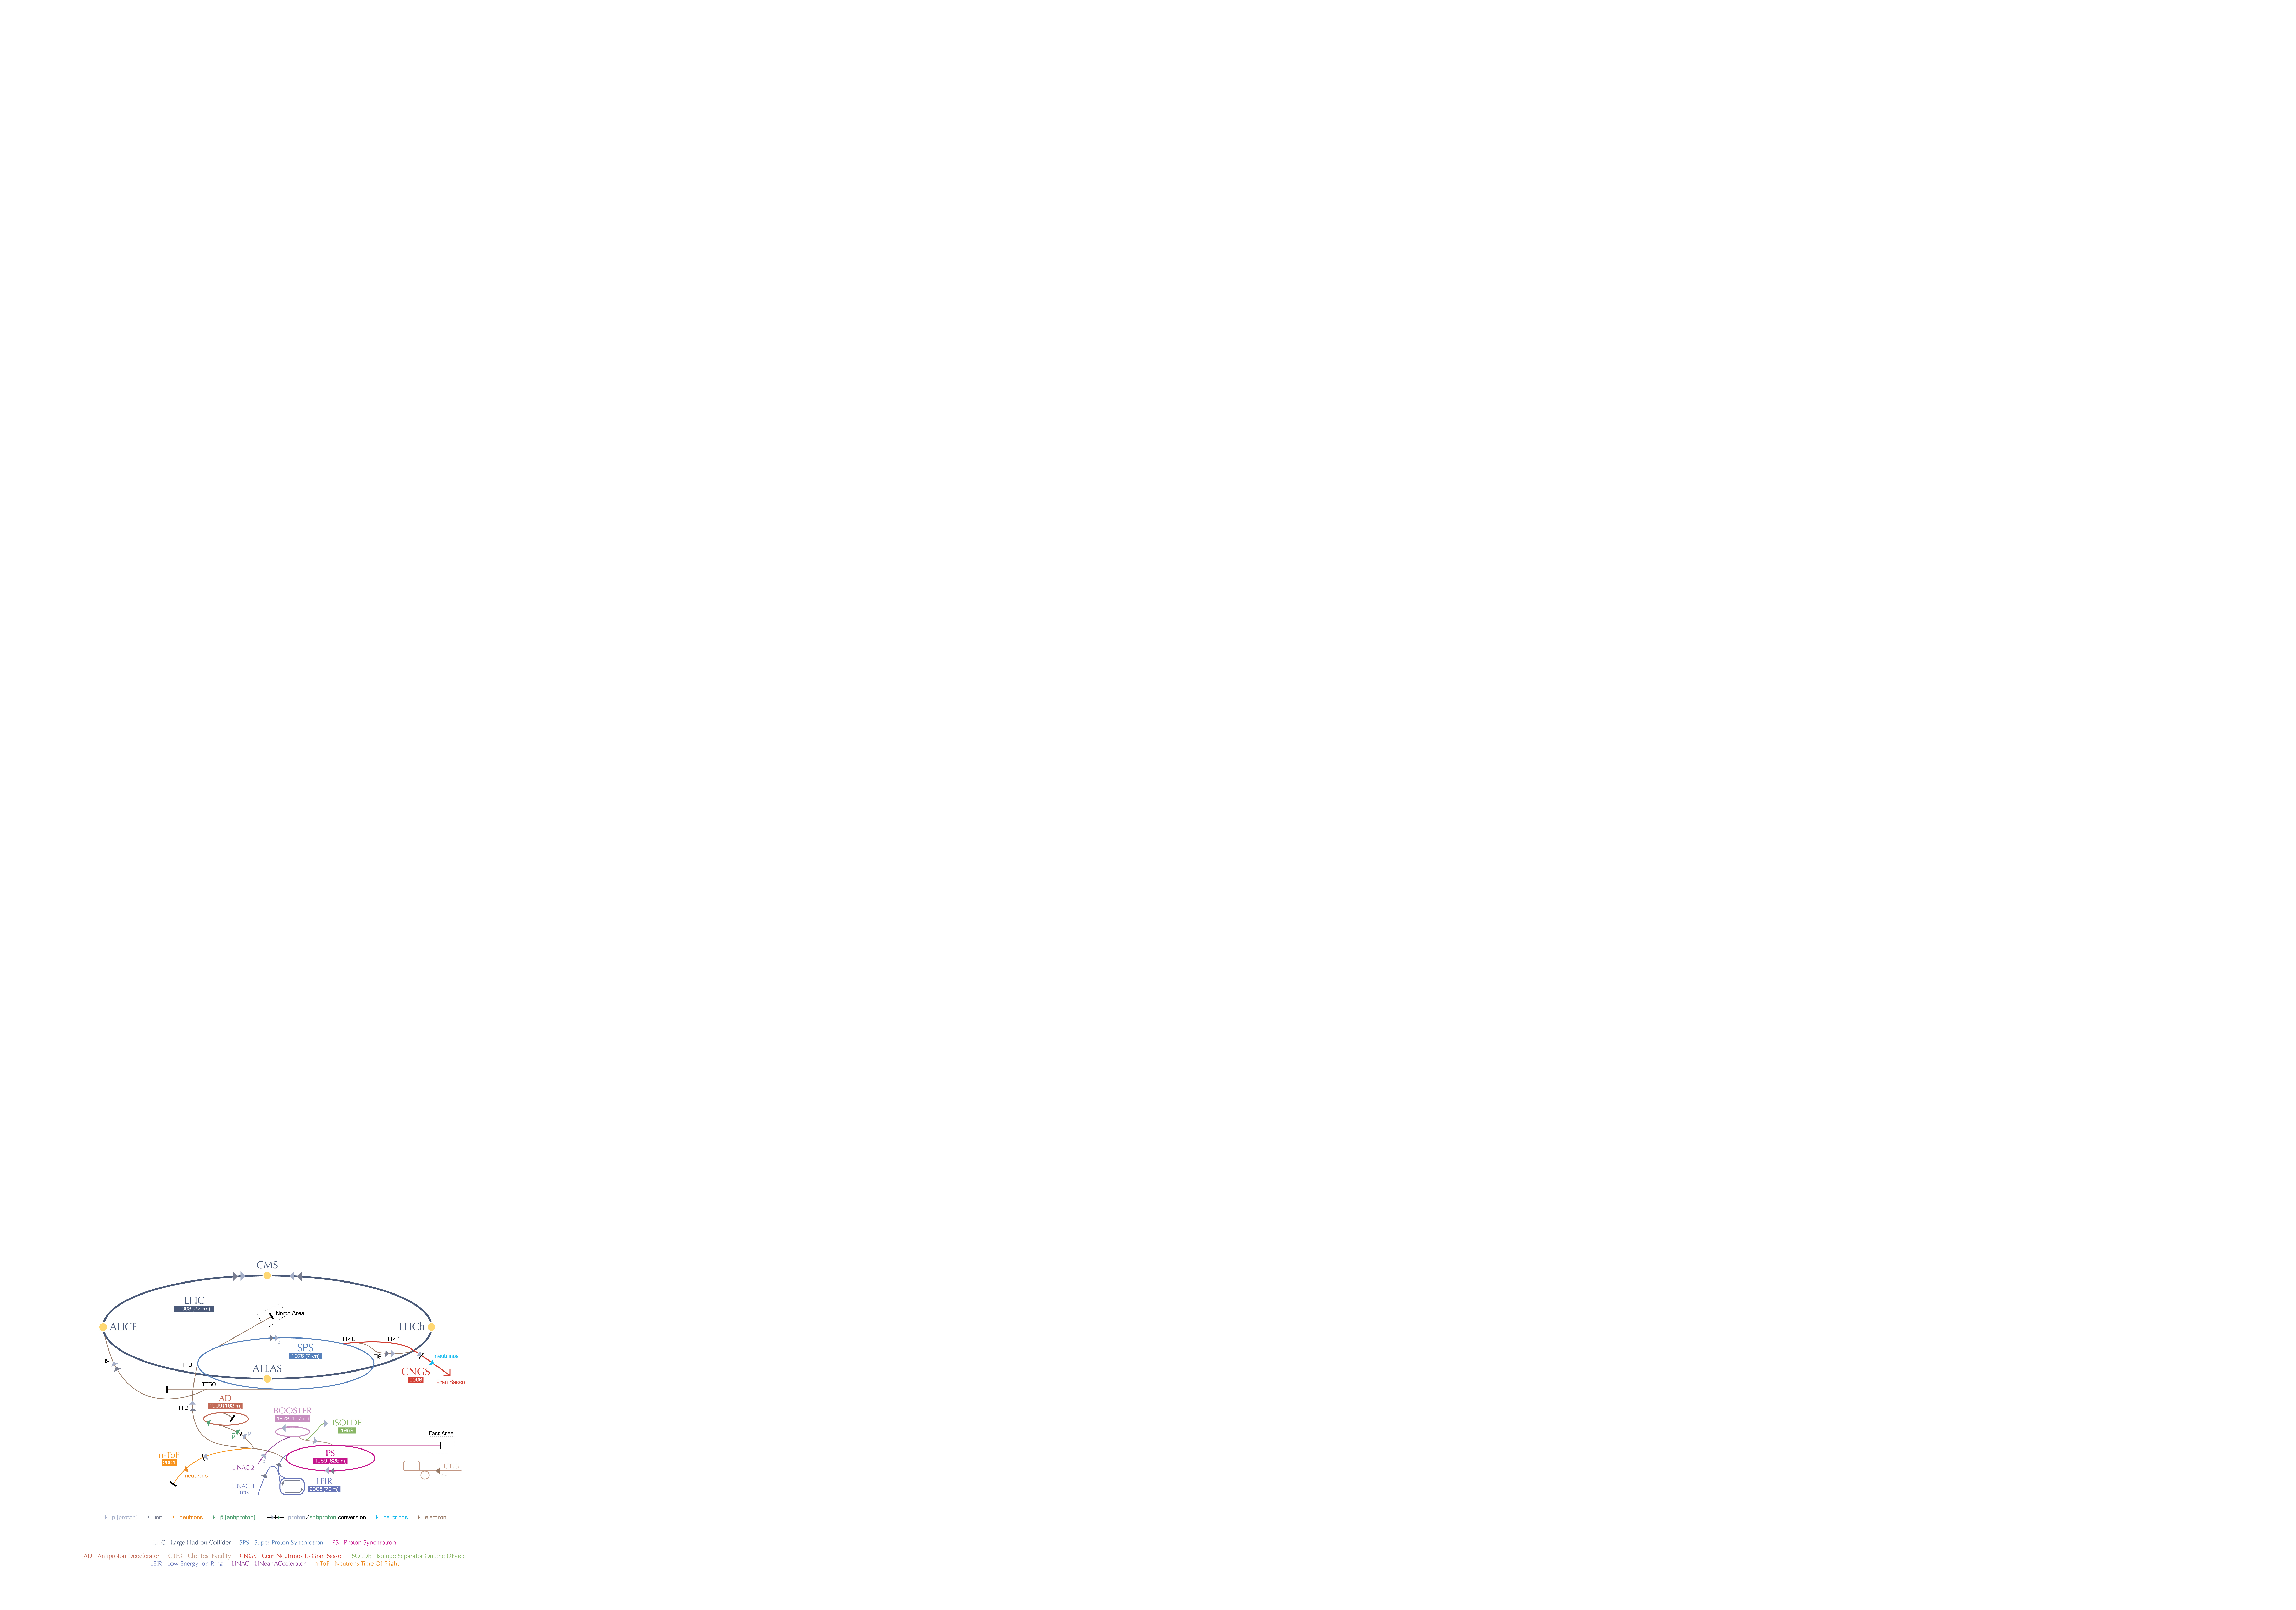
\includegraphics[width=\textwidth]{Figures/Detector/CERNschematic.pdf}
  \caption[The CERN accelerator complex.]
  {The LHC and its experiments within the CERN accelerator complex.
  Figure taken from Ref.~\cite{CERNcomplex}.}
  \label{fig:detector_CERNschematic}
\end{figure}

The LHC design parameters allow for proton-proton collisions to occur at a maximum centre-of-mass energy of 14\,TeV with an instantaneous luminosity of up to $10^{34}\,\textrm{cm}^{-2}\,\textrm{s}^{-1}$.
Prior to being injected into the LHC beam pipes, bunches of protons pass are accelerated in several stages. 
First, protons are obtained by stripping the electrons from hydrogen atoms using a strong electric field.
The protons produced are then accelerated up to an energy of 50 MeV by Linear Accelerator 2 (LINAC 2).
LINAC 2 leads into the Proton Synchrotron Booster (PSB), where they reach an energy of 1.4 GeV before passing into the Proton Synchrotron (PS).
Here the beam is accelerated up to 25 GeV before being transferred to the Super Proton Synchtroron (SPS).
The SPS is the last step before the protons enter the LHC itself at an energy of 540 GeV.
Therefore the LHC is responsible for the final acceleration from 540 GeV to the full energy.
Thus far, the energy reached for stable operation is 6.5\,TeV per beam; the full design energy is expected to be achieved in future.

The key components of the LHC are its 1232 main dipole magnets, 392 main quadrupole magnets and 16 radiofrequency (RF) cavities.
Superfluid helium cools the dipole magnets to 1.9K, at which temperature they produce the 8.3T magnetic field required to keep the beams in circular orbit.
Quadropole magnets are used principally to focus the beams near the interaction points, which increases the probability of a high-energy proton-proton collision.
The RF cavities deliver an accelerating field of 5MV/m at a frequency of 400MHz, and furthermore maintain the shape of the 2808 proton bunches per beam.
Collisions occur at the four interaction points, where bunches are induced to collide at a frequency of 25ns. 

The operation of the LHC to date has comprised two separate runs.
Run 1 commenced in 2010 with $\sqrt{s}$ = 7\,TeV, continuing into 2011 at the same centre-of-mass energy to give a total of 6.1\,\fb of data.
In 2012 this was increased to 8\,TeV, and a total of 23.3\,\fb of data were collected.
Analyses based upon this Run 1 dataset were able to discover the Higgs boson.
After a shutdown for upgrades to the machine, Run 2 ran from 2015 to 2018 at a constant 13\,TeV centre-of-mass energy.
The LHC was able to exceed its design luminosity in each of the years, eventually levelling the luminosity at $2\times10^{34}\,\textrm{cm}^{-2}\,\textrm{s}^{-1}$ for the majority of 2018 operations.
A number of additional inleastic proton-proton collisions in addition to a collision of interest, known as pileup, occur at a rate proportional to the instantaneous luminosity.
The mean number of pileup events was 27 per bunch crossing in 2016, and 37 in both 2017 and 2018 data-taking.
Figure \ref{fig:detector_Run1andRun2lumi} summarises the data collected in each year.
The latest \Hgg results on which this thesis is based have utilised the 2016 and 2017 datasets; 
plans for the final Run 2 result combining the 2016-2018 datasets are described in Chapter ~\ref{chap:conclusion}.
Furthermore, future upgrades to both the LHC and the CMS detector are discussed in Chapter~\ref{chap:hgcal}.

\begin{figure}[h!]
  \centering
  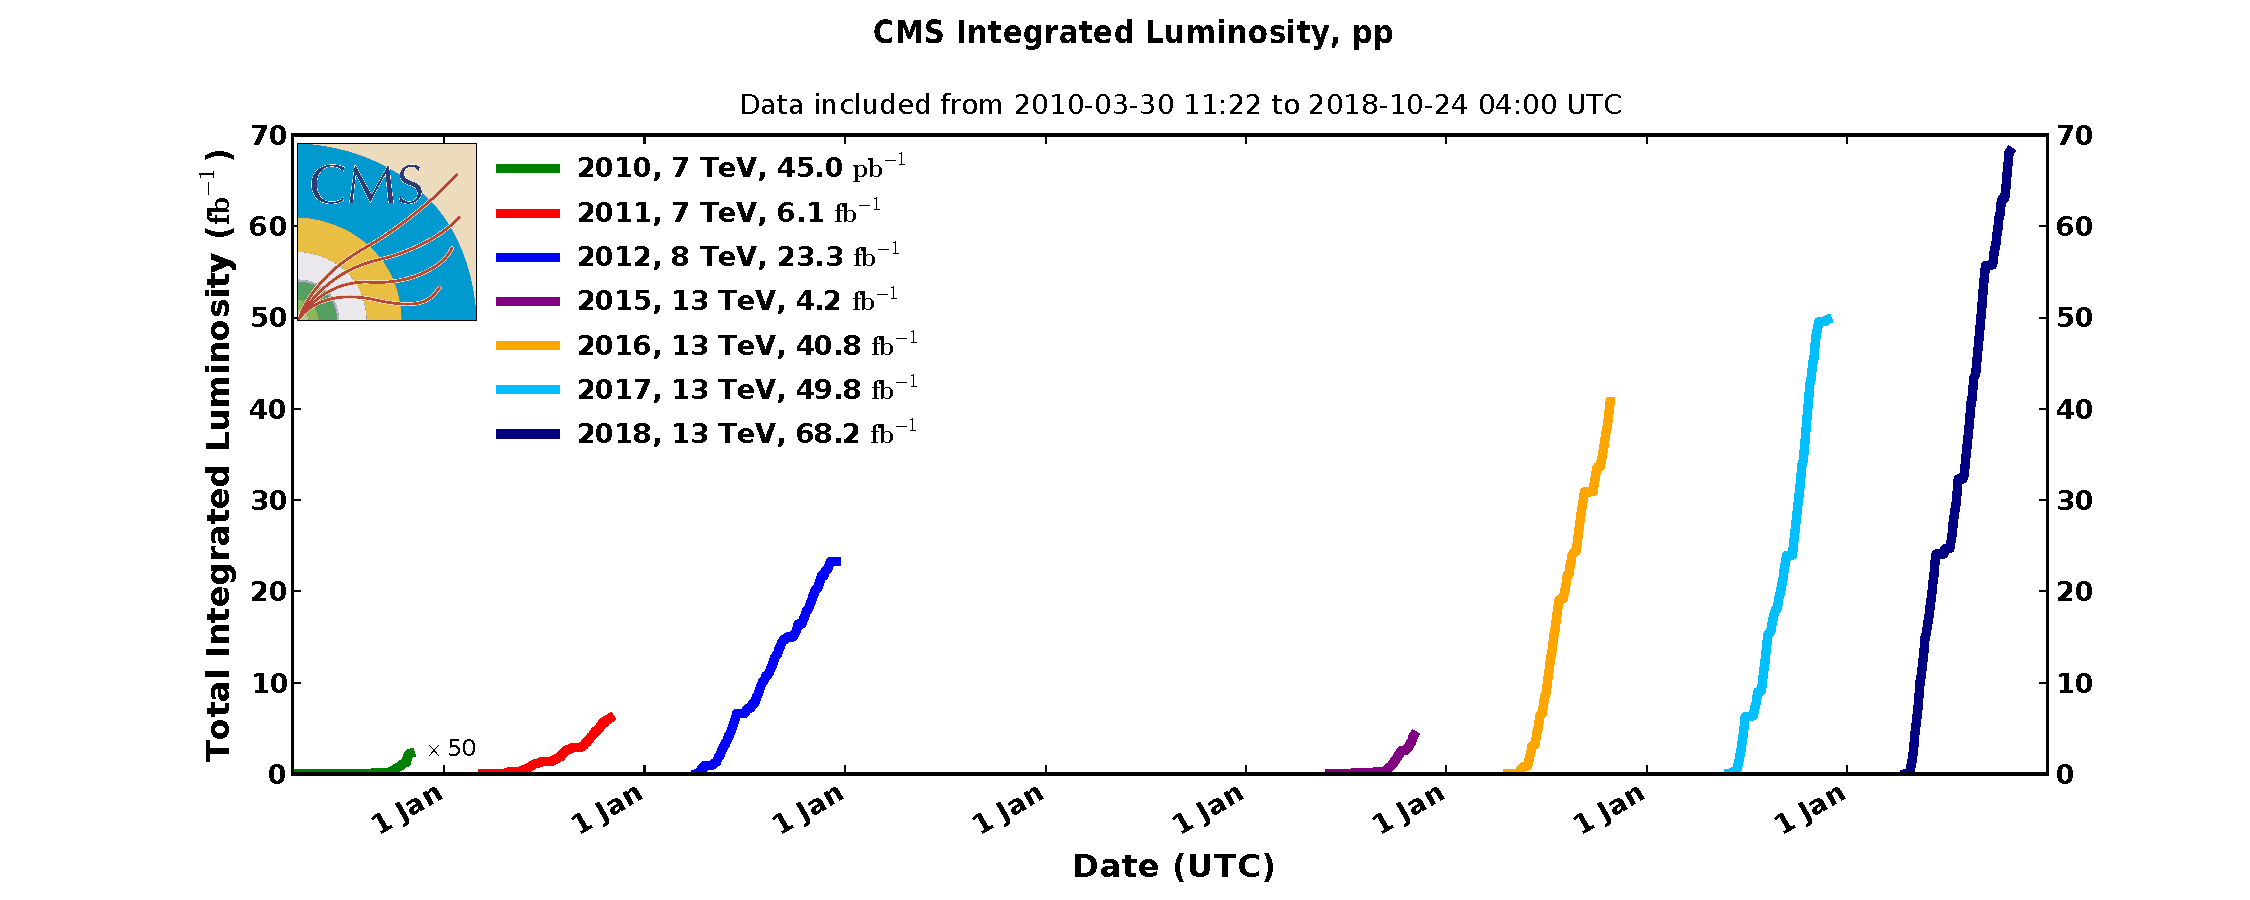
\includegraphics[width=\textwidth]{Figures/Detector/Run1andRun2lumi.pdf}
  \caption[LHC integrated luminosity and centre-of-mass energy per year.]
  {The integrated luminosity and centre-of-mass energy for each year of LHC operation.
  Figure taken from Ref.~\cite{CMSLumiPublic}.}
  \label{fig:detector_Run1andRun2lumi}
\end{figure}

\section{The CMS detector}

CMS is a general purpose detector~\cite{CMSdetector} designed to capture the full range of objects required to achieve the goals of the LHC physics programme.
The apparatus must be able to cope with very high pileup events at a very high rate; around 1000 charged particles are produced every 25\,ns.
Fine spatial and temporal granularity is required to obtain the sufficiently low occupancy necessary to perform well in these conditions.
The resulting quantity of detector channels presents challenges for the detector electronics.
Furthermore, the detector and its electronics must withstand high doses of radiation and fluence.

In addition to these technical constraints, CMS has four key physics requirements.
These are summarised as:
\begin{itemize}
  \item{\textbf{Muon identification and resolution} 
  muons must be identified and well-measured over wide range in energy and angle, 
  with good dimuon mass resolution and the capability to accurately determine their charge.
  This is veyr important for Higgs searches, particularly in the $ZZ$ decay channel.}
  \item{\textbf{Charged particle measurement}
  good momentum resolution along with efficient reconstruction and triggering on $\tau$ particles and $b$-jets.
  High jet reconstruction performance is essential in the majority of physics measurements.}
  \item{\textbf{Electromagnetic energy resolution}
  good energy resolution and isolation for electrons and photons, whilst maintaining high acceptance.
  These properties are vital for Higgs measurements, especially in the diphoton decay channel.}
  \item{\textbf{Missing energy resolution}
  accurate missing energy calculation and mass resolution of dijet objects.
  Missing energy is the key signature in many analyses searching for supersymmetry.}
\end{itemize}

The design of CMS fulfils each of these requirements.
The hermetic detector is cyclindrical in shape, housing the eponymous 4\,T solenoidal magnet in the central section.
Its other key components include the silicon tracker, homogeneous crystal electromagnetic calorimeter and a sampling hadronic calorimeter.
The tracker and calorimeters lie inside the bore of the magnet coil; the muon detection system is instead interleaved with the return yoke.
Each of these subsystems is displayed in Figure~\ref{fig:detector_CMSschematic}, and described in detail in the remainder of this chapter.

\begin{figure}[h!]
  \centering
  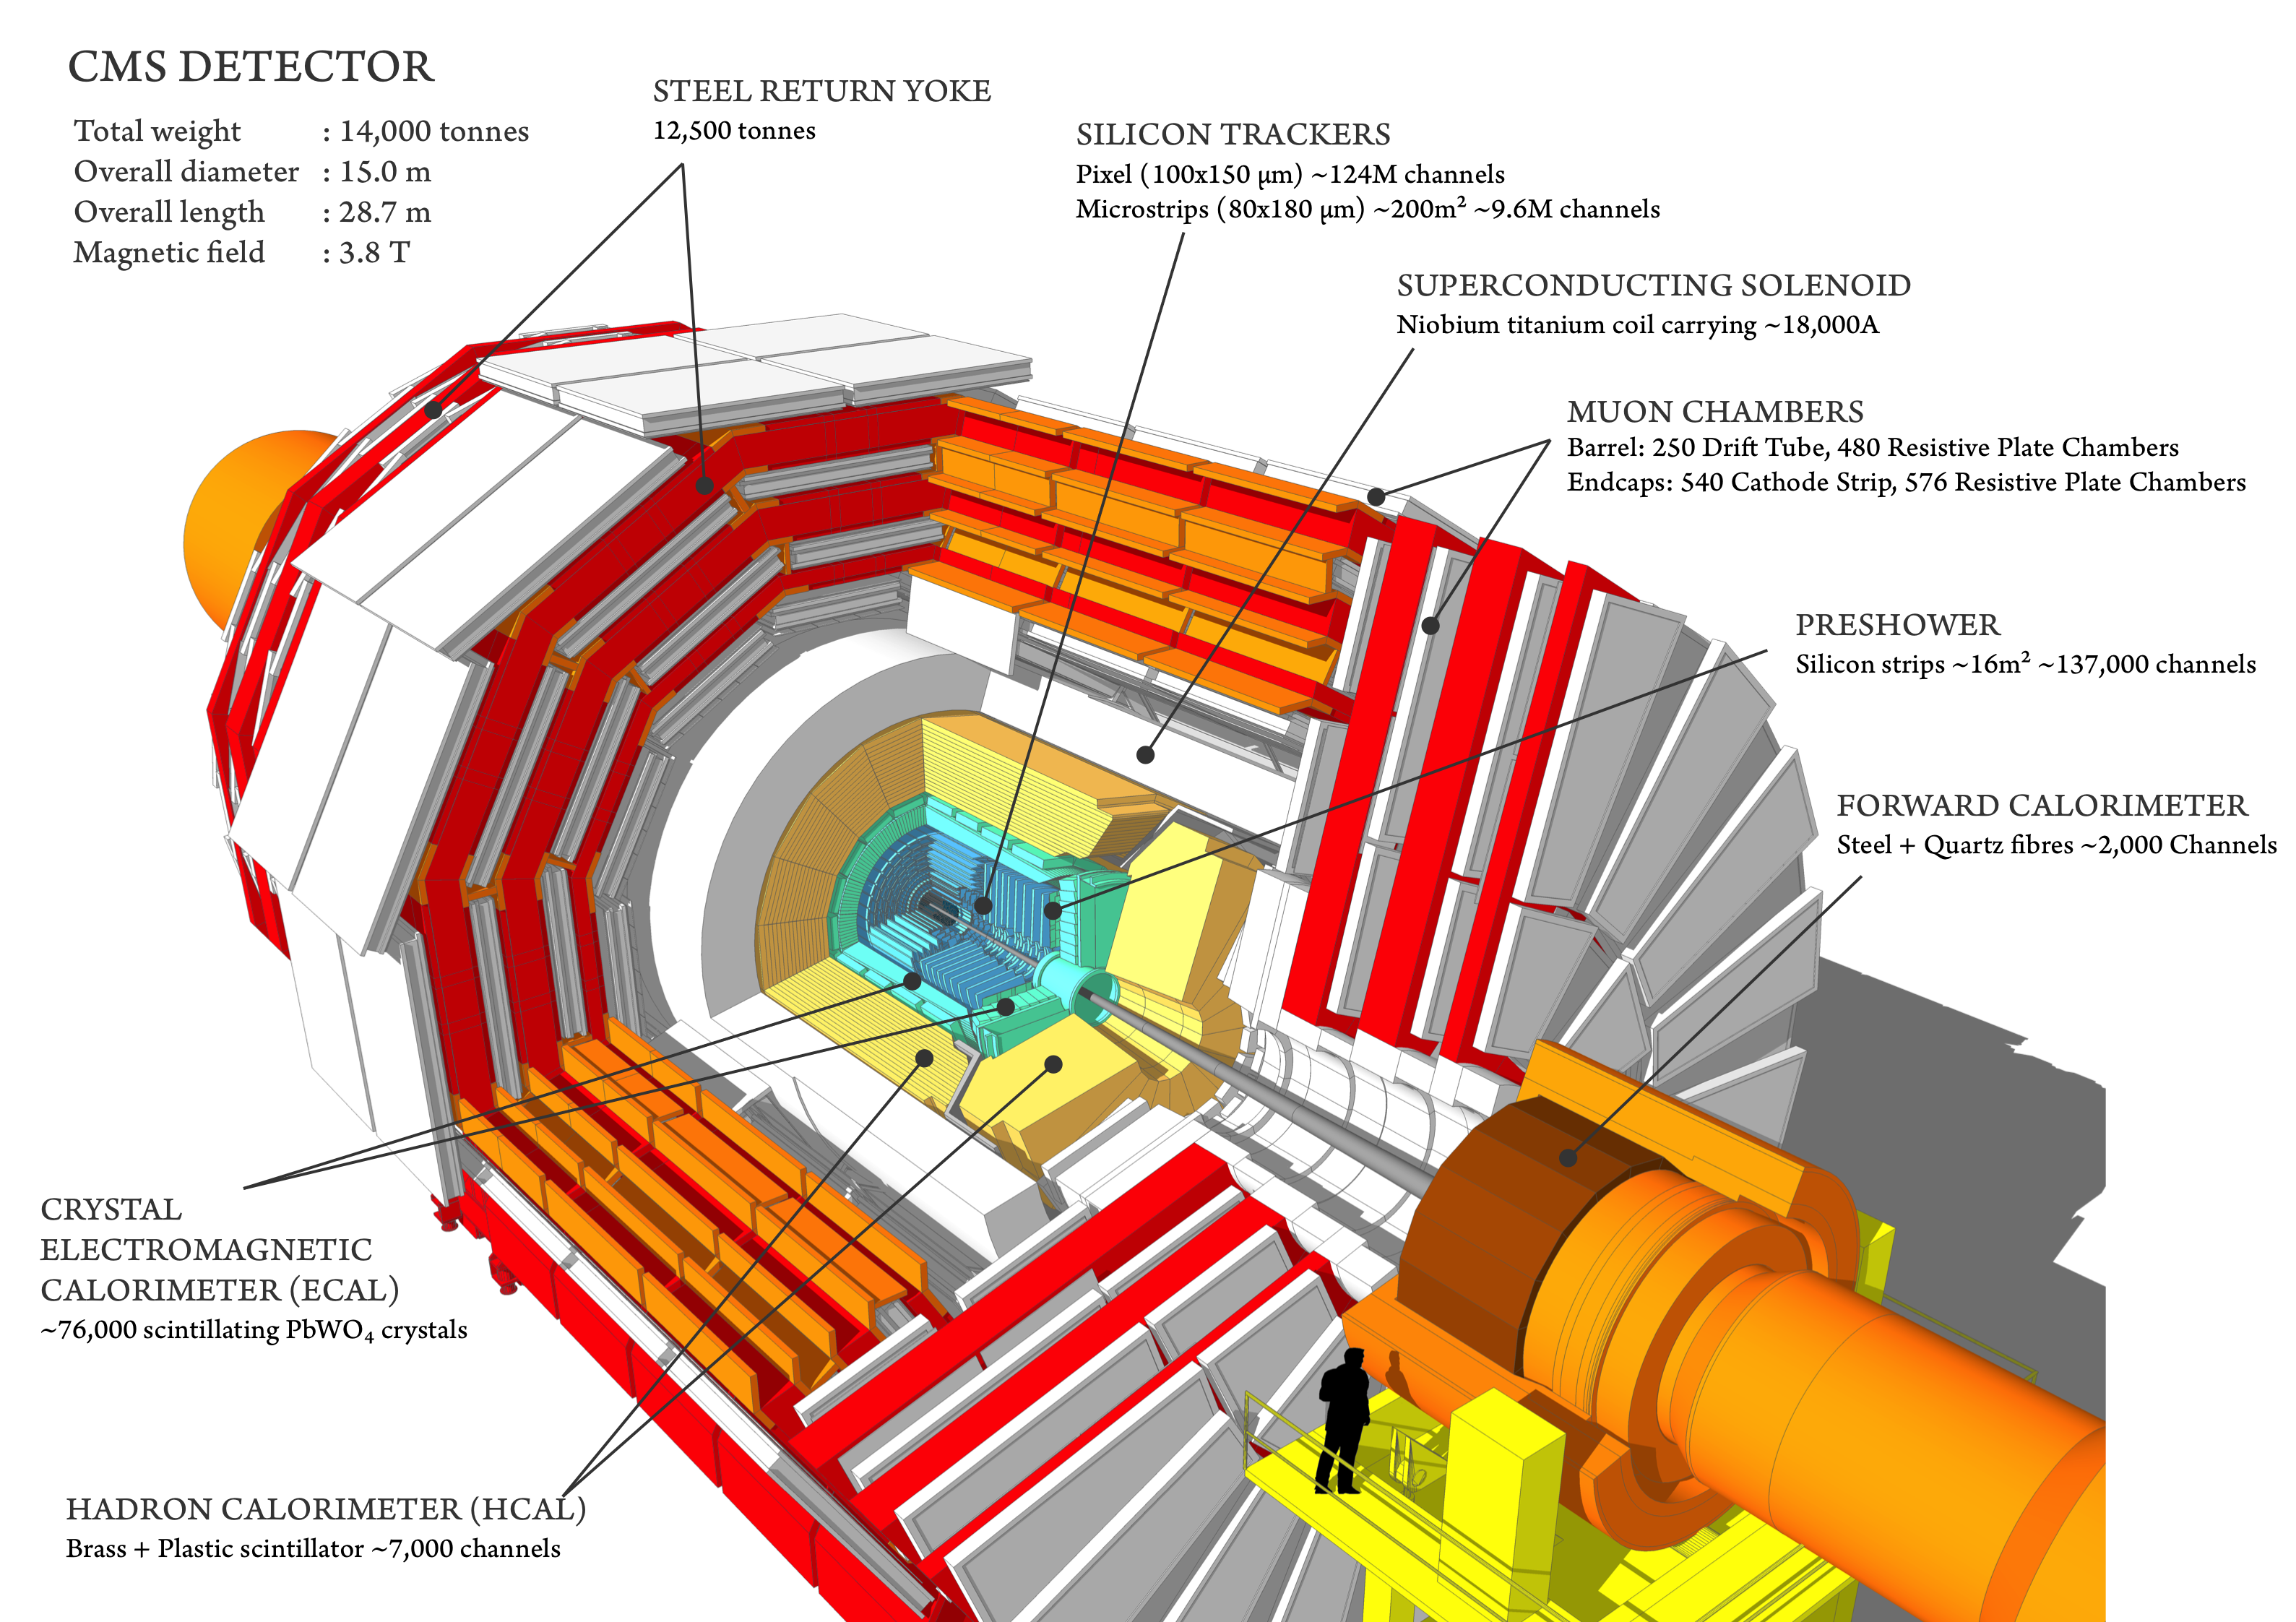
\includegraphics[width=\textwidth]{Figures/Detector/CMSschematic.png}
  \caption[A schematic view of CMS.]
  {A schematic view of the CMS detector.
  Part of the detector is cut away in order to display each subsystem.
  Figure taken from Ref.~\cite{SketchUp}.}
  \label{fig:detector_CMSschematic}
\end{figure}

A cylindrical cooordinate system is frequently to describe events within the CMS, with its centre at the nominal proton-proton interaction point.
The central part is referred to as the barrel, with two endcaps closing the cylinder.
The positive $z$-axis is defined to be parallel to the beampipe in the direction of the Jura mountains, anti-clockwise when viewed from above.
The azimuthal angle $\phi$ is measured from the $z$-axis, and polar angle $\theta$ from the plane perpendicular to the $z$-axis.
Other common quantities are: pseudorapidity, defined as $\eta = -\ln{\tan{\theta/2}}$; 
momentum in the direction transverse to the plane of the LHC, \pt; 
and the negative vector sum of particle energies, $E^{\textrm{miss}}_{T}$.
High pseudorapidity values, corresponding to a direction close to the beampipe, are referred to as being forward.

\subsection{Solenoid}

The central feature of the CMS detector is the superconducting solenoid, whose 220 tonne cold mass is maintained at 4.5\,K.%using liquid helium cooling - 1.8K redundancy
The coil of the magnet measures 6\,m in diameter, is 13\,m long, and provides a maximum field strength of 4\,T, storing  total energy of 1.6\,GJ.
During normal operation however the current is reduced to approximtely 95\% of its capacity, resulting in a field strength of 3.8\,T.
This ensures the longevity of the solenoid.
The magnetic flux is returned by a 10,000 tonne yoke, composed of three disk-like layers in both the barrel and endcaps.

The extremely high bending power of the CMS magnet enables precise measurement of charged particle tracks , 
and hence excellent momentum resolution up to very high particle momenta.
Its layout drives the design of the rest of the detector.

\subsection{Tracking}


\subsection{Electromagnetic calorimeter}
\subsection{Hadronic calorimeter}
\subsection{Muon system}
\subsection{Trigger system}
